% move all configuration stuff into includes file so we can focus on the content
\documentclass[aspectratio=169,hyperref={pdfpagelabels=false,colorlinks=true,linkcolor=white,urlcolor=blue},t]{beamer}

%%%%%%%%%%%%%%%%%%%%%%%%%%%%%%%%%%%%%%%%%%%%%%%%%%%%%%%%%%%%%%%%%%%%%%%%%%%%%%%%%%
%%%%%%%%%%%%%%%%%%%%%%%%%%%%%%%%%%%%%%%%%%%%%%%%%%%%%%%%%%%%%%%%%%%%%%%%%%%%%%%%%%
% packages
\usepackage{pict2e}
\usepackage{epic}
\usepackage{amsmath,amsfonts,amssymb}
\usepackage{units}
\usepackage{fancybox}
\usepackage[absolute,overlay]{textpos} 
\usepackage{media9} % avi2flv: "C:\Program Files\ffmpeg\bin\ffmpeg.exe" -i TuneFreqFilterbank.avi -b 600k -s 441x324 -r 15 -acodec copy TuneFreqFilterbank.flv
\usepackage{animate}
\usepackage{gensymb}
\usepackage{multirow}
\usepackage{silence}
\usepackage[backend=bibtex,style=ieee]{biblatex}
\AtEveryCitekey{\iffootnote{\tiny}{}}
\addbibresource{references}

%%%%%%%%%%%%%%%%%%%%%%%%%%%%%%%%%%%%%%%%%%%%%%%%%%%%%%%%%%%%%%%%%%%%%%%%%%%%%%%%%%
%%%%%%%%%%%%%%%%%%%%%%%%%%%%%%%%%%%%%%%%%%%%%%%%%%%%%%%%%%%%%%%%%%%%%%%%%%%%%%%%%%
% relative paths
\graphicspath{{graph/}}


%%%%%%%%%%%%%%%%%%%%%%%%%%%%%%%%%%%%%%%%%%%%%%%%%%%%%%%%%%%%%%%%%%%%%%%%%%%%%%%%%%
%%%%%%%%%%%%%%%%%%%%%%%%%%%%%%%%%%%%%%%%%%%%%%%%%%%%%%%%%%%%%%%%%%%%%%%%%%%%%%%%%%
% units
\setlength{\unitlength}{1mm}

%%%%%%%%%%%%%%%%%%%%%%%%%%%%%%%%%%%%%%%%%%%%%%%%%%%%%%%%%%%%%%%%%%%%%%%%%%%%%%%%%%
%%%%%%%%%%%%%%%%%%%%%%%%%%%%%%%%%%%%%%%%%%%%%%%%%%%%%%%%%%%%%%%%%%%%%%%%%%%%%%%%%%
% theme & layout
\usetheme{Frankfurt}
\beamertemplatenavigationsymbolsempty
%\setbeamertemplate{frametitle}[smoothbars theme]
\setbeamertemplate{frametitle}
{
    \begin{beamercolorbox}[ht=1.8em,wd=\paperwidth]{frametitle}
        \vspace{-.1em}%
        \hspace{.2em}{\strut\insertframetitle\strut}
        
        \hspace{.2em}\small\strut\insertframesubtitle\strut
        %\hfill
        %
\includegraphics[height=.8cm,keepaspectratio]{CenterMusicTechnology-solid-2lines-white-CoAtag}
        
    \end{beamercolorbox}
    \begin{textblock*}{100mm}(11.6cm,.7cm)
        \includegraphics[height=.8cm,keepaspectratio]{logo_GTCMT_black}
    \end{textblock*}
}

% set this to ensure bulletpoints without subsections
\usepackage{remreset}
\makeatletter
\@removefromreset{subsection}{section}
\makeatother
\setcounter{subsection}{1}

%---------------------------------------------------------------------------------
% appearance
\setbeamercolor{structure}{fg=gtgold}
\setbeamercovered{transparent} %invisible
\setbeamercolor{bibliography entry author}{fg=black}
\setbeamercolor*{bibliography entry title}{fg=black}
\setbeamercolor*{bibliography entry note}{fg=black}

%\usepackage{pgfpages}
%\setbeameroption{show notes}
%\setbeameroption{show notes on second screen=right}
%---------------------------------------------------------------------------------
% fontsize
\let\Tiny=\tiny

%%%%%%%%%%%%%%%%%%%%%%%%%%%%%%%%%%%%%%%%%%%%%%%%%%%%%%%%%%%%%%%%%%%%%%%%%%%%%%%%%%
%%%%%%%%%%%%%%%%%%%%%%%%%%%%%%%%%%%%%%%%%%%%%%%%%%%%%%%%%%%%%%%%%%%%%%%%%%%%%%%%%%
% warnings
\pdfsuppresswarningpagegroup=1
\WarningFilter{biblatex}{Patching footnotes failed}
\WarningFilter{latexfont}{Font shape}
\WarningFilter{latexfont}{Some font shapes}
\WarningFilter{gensymb}{Not defining}


%%%%%%%%%%%%%%%%%%%%%%%%%%%%%%%%%%%%%%%%%%%%%%%%%%%%%%%%%%%%%%%%%%%%%%%%%%%%%%%%%%
%%%%%%%%%%%%%%%%%%%%%%%%%%%%%%%%%%%%%%%%%%%%%%%%%%%%%%%%%%%%%%%%%%%%%%%%%%%%%%%%%%
% title information
\title[]{Introduction to Audio Content Analysis}   
\author[alexander lerch]{alexander lerch} 
%\institute{~}
%\date[Alexander Lerch]{}
\titlegraphic{\vspace{-16mm}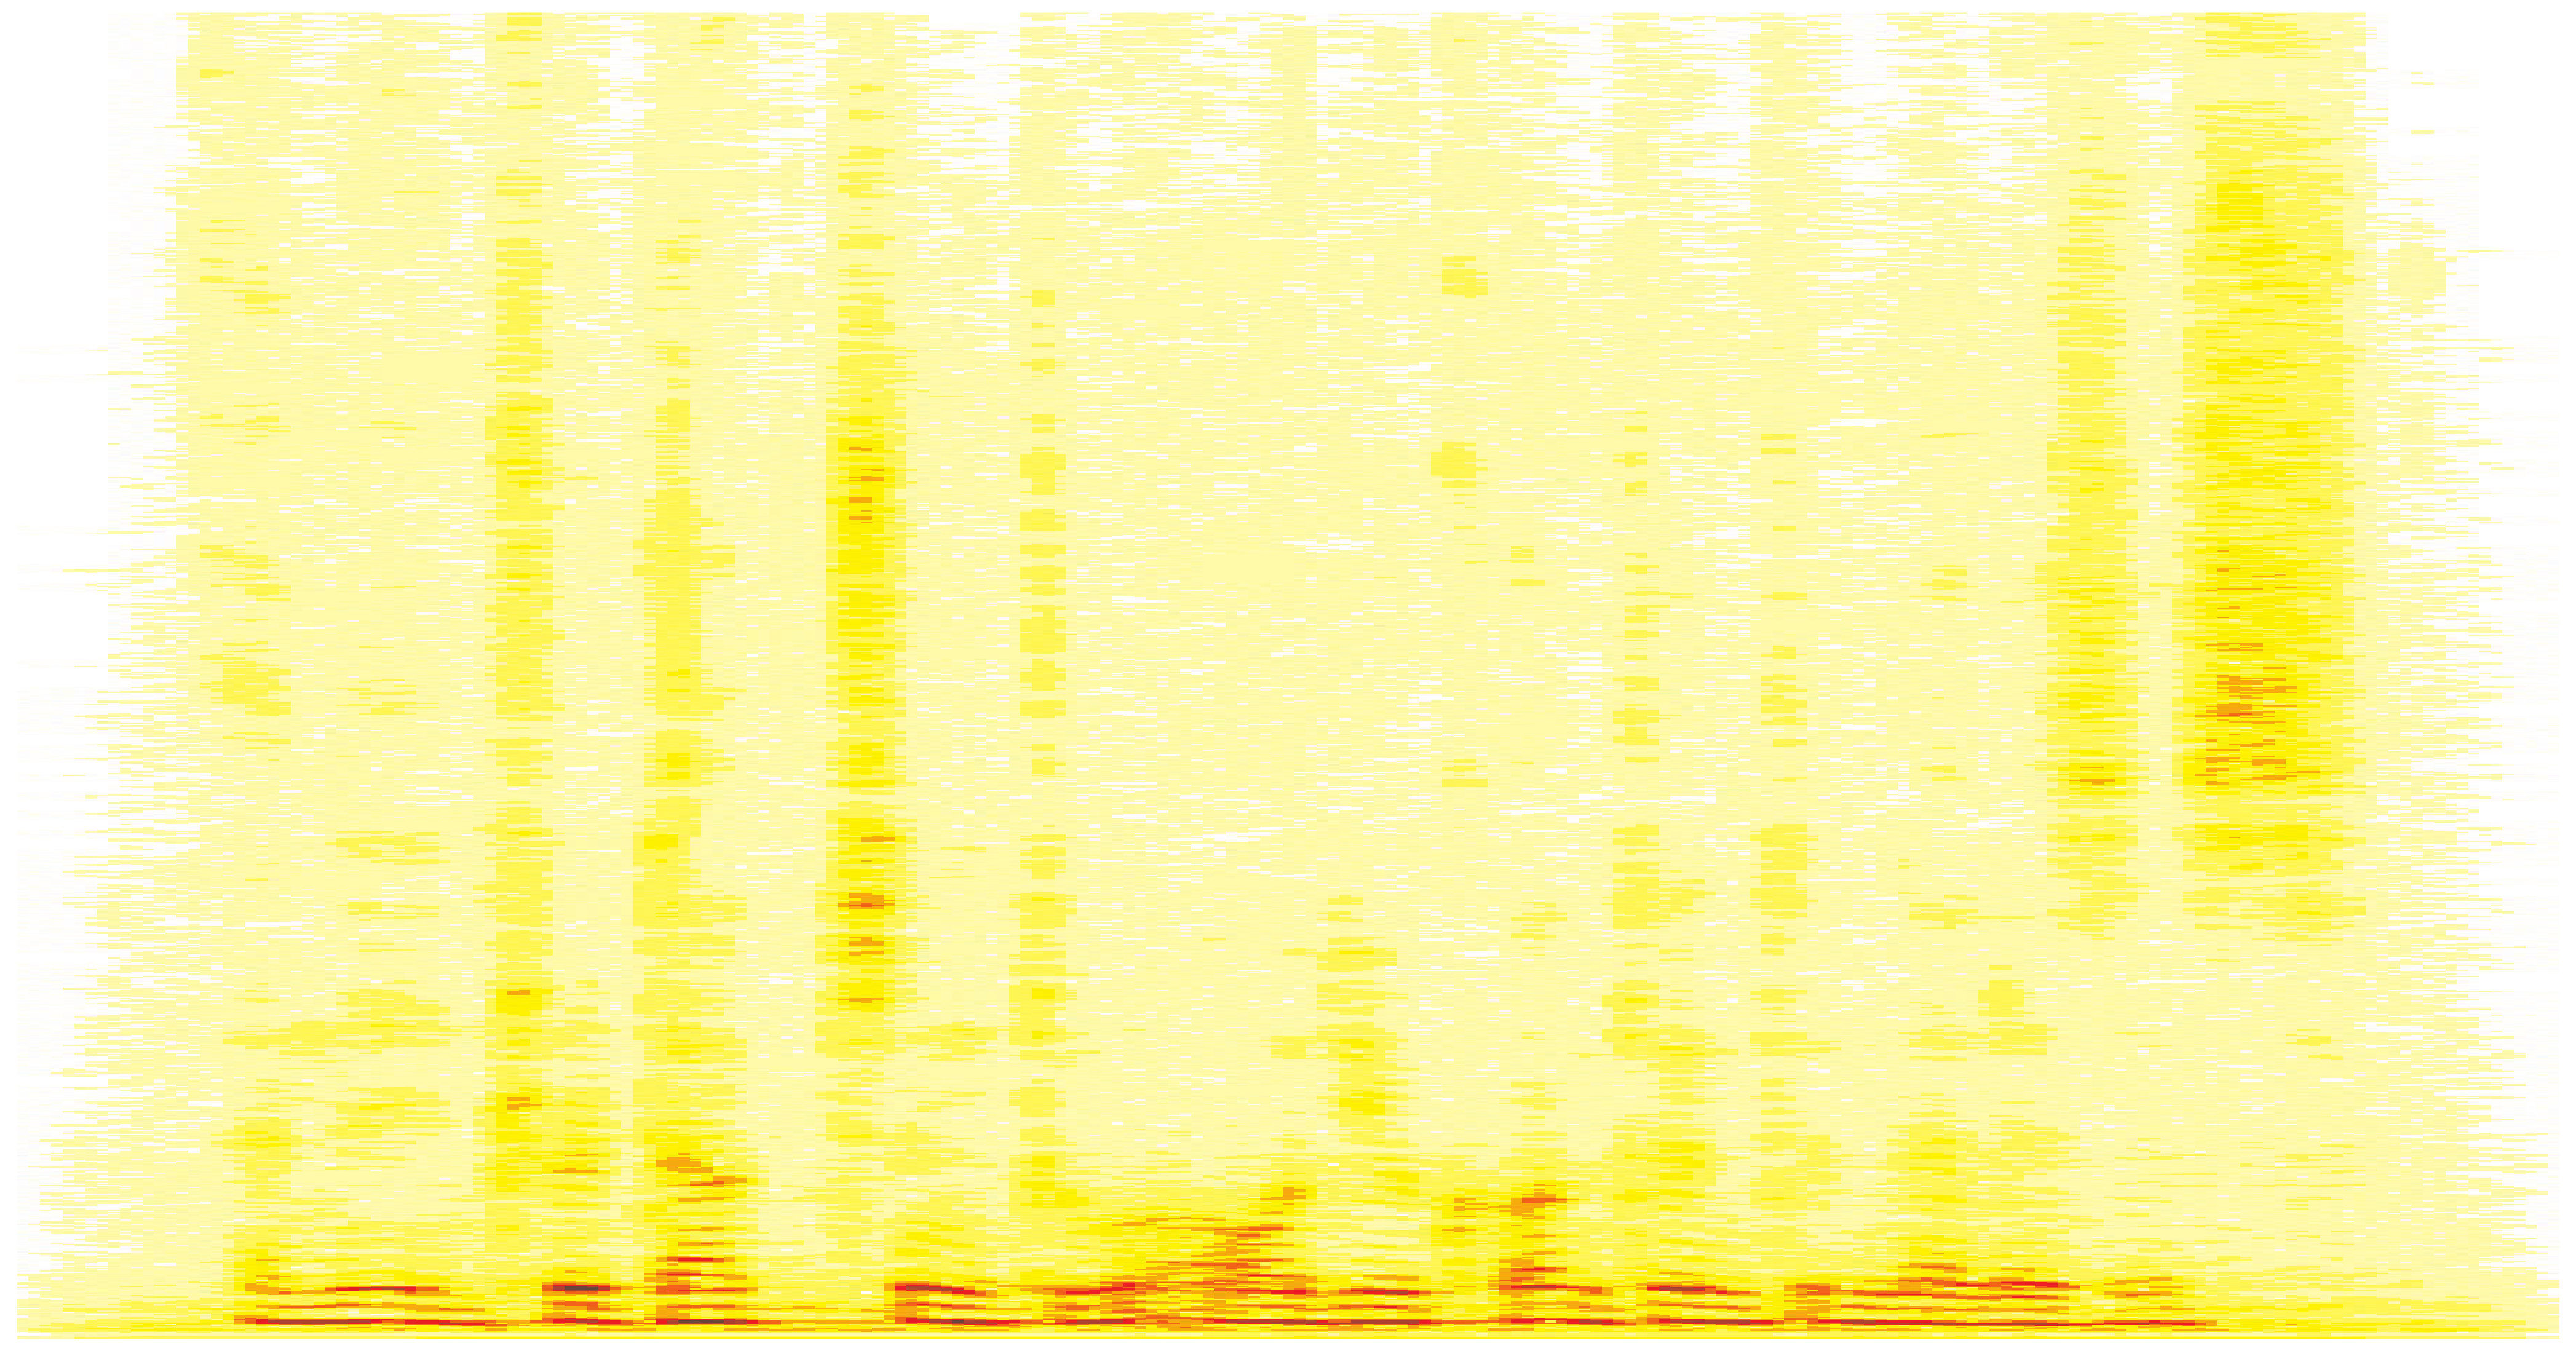
\includegraphics[width=\textwidth,height=3cm]{title}}

%%%%%%%%%%%%%%%%%%%%%%%%%%%%%%%%%%%%%%%%%%%%%%%%%%%%%%%%%%%%%%%%%%%%%%%%%%%%%%%%%%
%%%%%%%%%%%%%%%%%%%%%%%%%%%%%%%%%%%%%%%%%%%%%%%%%%%%%%%%%%%%%%%%%%%%%%%%%%%%%%%%%%
% colors
\definecolor{gtgold}{HTML}{E0AA0F} %{rgb}{0.88,0.66,1,0.06} [234, 170, 0]/256

%%%%%%%%%%%%%%%%%%%%%%%%%%%%%%%%%%%%%%%%%%%%%%%%%%%%%%%%%%%%%%%%%%%%%%%%%%%%%%%%%%
%%%%%%%%%%%%%%%%%%%%%%%%%%%%%%%%%%%%%%%%%%%%%%%%%%%%%%%%%%%%%%%%%%%%%%%%%%%%%%%%%%
% math
\DeclareMathOperator*{\argmax}{argmax}
\DeclareMathOperator*{\argmin}{argmin}
\DeclareMathOperator*{\atan}{atan}
\DeclareMathOperator*{\arcsinh}{arcsinh}
\DeclareMathOperator*{\sign}{sign}
\DeclareMathOperator*{\tcdf}{tcdf}
\DeclareMathOperator*{\si}{sinc}
\DeclareMathOperator*{\princarg}{princarg}
\DeclareMathOperator*{\arccosh}{arccosh}
\DeclareMathOperator*{\hwr}{HWR}
\DeclareMathOperator*{\flip}{flip}
\DeclareMathOperator*{\sinc}{sinc}
\DeclareMathOperator*{\floor}{floor}
\newcommand{\e}{{e}}
\newcommand{\jom}{\mathrm{j}\omega}
\newcommand{\jOm}{\mathrm{j}\Omega}
\newcommand   {\mat}[1]    		{\boldsymbol{\uppercase{#1}}}		%bold
\renewcommand {\vec}[1]    		{\boldsymbol{\lowercase{#1}}}		%bold

%%%%%%%%%%%%%%%%%%%%%%%%%%%%%%%%%%%%%%%%%%%%%%%%%%%%%%%%%%%%%%%%%%%%%%%%%%%%%%%%%%
%%%%%%%%%%%%%%%%%%%%%%%%%%%%%%%%%%%%%%%%%%%%%%%%%%%%%%%%%%%%%%%%%%%%%%%%%%%%%%%%%%
% media9
\newcommand{\includeaudio}[1]{{\includemedia[
                        addresource=audio/#1.mp3,
                        width=5mm,
                        height=5mm,
                        activate=onclick,
                        flashvars={
                            source=audio/#1.mp3  
                            &autoPlay=true
                        }]
                        {
\includegraphics[width=5mm, height=5mm]{SpeakerIcon}}
                        {APlayer.swf}}}
\newcommand{\audioautoplay}[1]{{\begin{center}\includemedia[
                            addresource=audio/#1.mp3,
                            width=.1\linewidth,
                            height=.01\linewidth,
                            activate=pageopen,
                            flashvars={
                                source=audio/#1.mp3  
                                &autoPlay=true
                            }]
                            {}
                            {APlayer.swf}\end{center}}}

\newcommand{\includevideo}[1]{{\begin{center}\includemedia[
                        addresource=video/#1.mp4,
                        width=0.8\linewidth,
                        height=0.4\linewidth,
                        activate=onclick,
                        flashvars={
                            source=video/#1.mp4  
                            &autoPlay=true
                        }]
                        {}
                        {VPlayer.swf}\end{center}}}
\newcommand{\videowithmatlab}[1]{{\begin{center}\includemedia[
                        addresource=video/animate#1.mp4,
                        width=0.8\linewidth,
                        height=0.4\linewidth,
                        activate=onclick,
                        flashvars={
                            source=video/animate#1.mp4  
                            &autoPlay=true
                        }]
                        {}
                        {VPlayer.swf}\end{center}\addreference{matlab source: matlab/animate#1.m}}}
                        

%%%%%%%%%%%%%%%%%%%%%%%%%%%%%%%%%%%%%%%%%%%%%%%%%%%%%%%%%%%%%%%%%%%%%%%%%%%%%%%%%%
%%%%%%%%%%%%%%%%%%%%%%%%%%%%%%%%%%%%%%%%%%%%%%%%%%%%%%%%%%%%%%%%%%%%%%%%%%%%%%%%%%
% other commands
\newcommand{\question}[1]{%\vspace{-4mm}
                          \setbeamercovered{invisible}
                          \begin{columns}[T]
                            \column{.8\textwidth}
                                \textbf{#1}
                            \column{.2\textwidth}
                                \vspace{-8mm}
                                \begin{flushright}
                                     
\includegraphics[scale=.5]{question_mark}
                                \end{flushright}
                                \vspace{6mm}
                          \end{columns}\pause\vspace{-12mm}}

\newcommand{\toremember}[1]{%\vspace{-4mm}
                          \begin{columns}[T]
                            \column{.8\textwidth}
                                \textbf{#1}
                            \column{.2\textwidth}
                                \vspace{-4mm}
                                \begin{flushright}
                                     
\includegraphics[scale=.5]{exclamation_mark}
                                \end{flushright}
                                \vspace{6mm}
                          \end{columns}\vspace{-6mm}}

\newcommand{\matlabexercise}[1]{%\vspace{-4mm}
                          \setbeamercovered{invisible}
                          \begin{columns}[T]
                            \column{.8\textwidth}
                                \textbf{matlab exercise}: #1
                            \column{.2\textwidth}
                                \begin{flushright}
                                     
\includegraphics[scale=.5]{logo_matlab}
                                \end{flushright}
                                %\vspace{6mm}
                          \end{columns}}

\newcommand{\addreference}[1]{  
                  
                    \begin{textblock*}{\baselineskip }(1.12\textwidth,.3\textheight) %(1.15\textwidth,.4\textheight)
                        \rotatebox{90}{\tiny {#1}}
                    \end{textblock*}}
                    
\newcommand{\figwithmatlab}[1]{
                    \begin{figure}
                        \centering
                        \includegraphics{#1}
                        %\label{fig:#1}
                    \end{figure}
                    
                    \addreference{matlab source: \href{https://github.com/alexanderlerch/ACA-Slides/blob/master/matlab/display#1.m}{matlab/display#1.m}}}
\newcommand{\figwithref}[2]{
                    \begin{figure}
                        \centering
                        \includegraphics{#1}
                        \label{fig:#1}
                    \end{figure}
                    
                    \addreference{#2}}  
                                    
\newcommand{\inserticon}[1]{

                    \begin{textblock*}{100mm}(14.5cm,7.5cm)
                        \includegraphics[height=.8cm,keepaspectratio]{#1}
                    \end{textblock*}}            

%%%%%%%%%%%%%%%%%%%%%%%%%%%%%%%%%%%%%%%%%%%%%%%%%%%%%%%%%%%%%%%%%%%%%%%%%%%%%%%%%%
%%%%%%%%%%%%%%%%%%%%%%%%%%%%%%%%%%%%%%%%%%%%%%%%%%%%%%%%%%%%%%%%%%%%%%%%%%%%%%%%%%
% counters
\newcounter{i}
\newcounter{j}
\newcounter{iXOffset}
\newcounter{iYOffset}
\newcounter{iXBlockSize}
\newcounter{iYBlockSize}
\newcounter{iYBlockSizeDiv2}
\newcounter{iDistance}



\subtitle{Module 5.5: Non-negative Matrix Factorization for Fundamental Frequency Detection}

%%%%%%%%%%%%%%%%%%%%%%%%%%%%%%%%%%%%%%%%%%%%%%%%%%%%%%%%%%%%%%%%%%%%%%%%%%%%
\begin{document}
    % generate title page
	

\begin{frame}
    \titlepage
    %\vspace{-5mm}
    \begin{flushright}
        \href{http://www.gtcmt.gatech.edu}{\includegraphics[height=.8cm,keepaspectratio]{logo_GTCMT_black}}
    \end{flushright}
\end{frame}


    \section[overview]{lecture overview}
        \begin{frame}{introduction}{overview}
            \begin{block}{corresponding textbook section}
                    \href{http://ieeexplore.ieee.org/xpl/articleDetails.jsp?arnumber=6331122}{Chapter 5~---~Tonal Analysis}: pp.~106
            \end{block}

            \begin{itemize}
                \item   \textbf{lecture content}
                    \begin{itemize}
                        \item   introduction to NMF
                        \item   objective function and update rules
                    \end{itemize}
                \bigskip
                \item<2->   \textbf{learning objectives}
                    \begin{itemize}
                        \item   describe the process of NMF
                        \item   discuss the pros and cons of using NMF of polyphonic pitch detection
                        \item   apply NMF to a simple audio file and interpret the results
                    \end{itemize}
            \end{itemize}
            \inserticon{directions}
        \end{frame}

    \section[intro]{introduction}
        \begin{frame}{non-negative matrix factorization}{introduction}
            \begin{itemize}
                \item   \textbf{Non-negative Matrix Factorization (NMF)}\\
                Given a $m \times n$ matrix $V$, find a $m \times r$ matrix $W$ and a $r \times n$ matrix $H$ such that
                \begin{equation*}
                V \approx WH
                \end{equation*}
                \begin{itemize}
                		\item all matrices must be non-negative
                		\item rank $r$ is usually smaller than $m$ and $n$
                \end{itemize}
              		                
                \bigskip
                \item<2->   \textbf{advantage of non-negativity?}
                    \begin{itemize}
                        \item<2->   additive model
                        \item<3->   relates to probability distributions
                        \item<4->   efficiency?
                    \end{itemize}
            \end{itemize}
        \end{frame}    
        
        \begin{frame}{non-negative matrix factorization}{overview}
           alternative formulation\footfullcite{cichocki_nmf_2009} to $V \approx WH$
            \begin{columns}
            \column{0.6\linewidth}
                \begin{equation*}
                V = \sum_{i = 1}^r w_{i} \cdot h_{i} + E
                \end{equation*}
            \column{0.6\linewidth}
			    \begin{itemize}
					\item  $V \in \mathbb{R}^{m \times n}$
					\item  $W = [w_{1}, w_{2}, ..., w_{r}] \in \mathbb{R}^{m \times r}$
					\item  $H  = [h_{1}, h_{2}, ..., h_{r}]^{T} \in \mathbb{R}^{r \times n}$
					\item  $E$ is the error matrix													   
				\end{itemize}			                   
            \end{columns}
            \begin{figure}
                    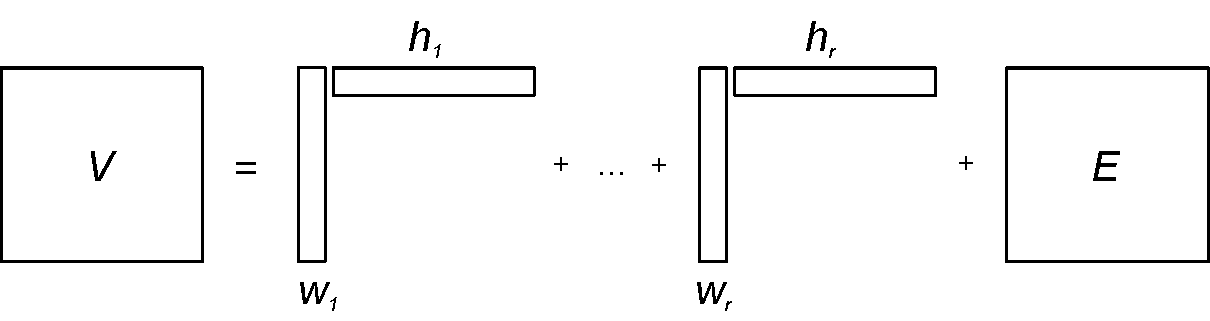
\includegraphics[scale=.35]{Nmf_Decomposition}
            \end{figure}
        \end{frame}        
        
    \section[objective function]{objective function}
        \begin{frame}{objective function}{distance and divergence}
            \begin{itemize}
                \item   task: \textbf{iteratively minimize objective function} $D(V || WH)$
                \bigskip
                \item   typical distance measures ($B = WH$):
                   \begin{itemize}
                        \item  squared Euclidean distance:\\
                        \begin{equation*}
                        D_\mathrm{EU}( V \parallel B) = \parallel V - B\parallel^{2} = \sum_{i j} (V_{i j} - B_{i j})^{2}
                        \end{equation*}
                       \item  generalized K-L divergence:\\
                       \begin{equation*}
                        D_\mathrm{KL}( V \parallel B) = \sum_{i j} (V_{i j} \log\left(\frac{V_{i j}}{B_{i j}}\right) - V_{i j} + B_{i j})
                        \end{equation*}		                
                        \bigskip
                        \item<2-> others\footfullcite{cichocki_nmf_2009}: Bregman Divergence, Alpha-Divergence, Beta-Divergence, \ldots 
                   \end{itemize}
            \end{itemize}
        
        \end{frame}          
    
        \begin{frame}{objective function}{gradient descent}
            \begin{itemize}
                \item   minimization of objective function

               \bigskip
            \item<2->  \textbf{gradient descent}: minimum can be found as zero of derivative
                       \begin{itemize}
                            \item  2D example: given a function $f(x_{1}, x_{2})$, find the minimum $x_{1} = a$ and $x_{2} = b$
                                \smallskip
                                \begin{enumerate}
                                    \item  initialize $x_{i}(0)$ with random numbers
                                    \item  update points iteratively:  
                                             \begin{equation*}
                                                 x_{i}(n+1) = x_{i}(n) - \alpha \cdot \frac{\partial f}{\partial x_{i}}, \quad i = [1, 2]
                                             \end{equation*}
                                \end{enumerate}
                            \bigskip
                            \item[$\Rightarrow$] as iteration number $n$ increases, $x_{1}$, $x_{2}$ will be closer to $a$, $b$.
                       \end{itemize}			   			   
            \end{itemize}
        \end{frame}    
          
        \begin{frame}{objective function}{additive vs.\ multiplicative update rules} 
           optimization of objective function\footfullcite{seung_nmf_2001} $D_\mathrm{EU}( V \parallel WH) = \parallel V - WH\parallel^{2}$
           \begin{itemize}
                \item  \textbf{additive} update rules:
                \begin{equation*}
                H \leftarrow H + \alpha \frac{\partial J}{\partial H} = H + \alpha [(W^{T}V) - (W^{T}WH)]
                \end{equation*}
                \begin{equation*}
                W \leftarrow W + \alpha \frac{\partial J}{\partial W} = W + \alpha [(VH^{T}) - (WHH^{T})]
                \end{equation*}
			   \item<2->  \textbf{multiplicative} update rules:
                \begin{equation*}
                H \leftarrow H \frac{(W^{T}H)}{(W^{T}WH)}
                \end{equation*}
                \begin{equation*}
                W \leftarrow W \frac{(VH^{T})}{(WHH^{T})}
                \end{equation*}
           \end{itemize}
        \end{frame}        
    
        \begin{frame}{objective function}{additional cost function constraints}
            \begin{itemize}
                \item   additional penalty terms (regularization terms) may be added to objective function
                \bigskip
                \item   example: sparsity in $W$ or $H$
                \begin{equation*}
                    D = \parallel V - WH\parallel^{2} + {\color{gtgold}{\alpha J_\mathrm{W}(W)}} + {\color{gtgold}{\beta J_\mathrm{H}(H)}}
                \end{equation*}
                \begin{itemize}
                    \item $\alpha,\beta$: coefficients for controlling degree of sparsity
                    \item $J_\mathrm{W}$ and $J_\mathrm{H}$: typically $L_{1},L_{2}$ norm 
                \end{itemize}
            \end{itemize}
        \end{frame}
              
    \section[example]{example}
        %\begin{frame}{in class exercise}{nmf for music transcription}
        %\matlabexercise{nmf based pitch tracking}
            %\begin{itemize}
                %\item   \textbf{unsupervised}  
                    %\begin{itemize}
                        %\item   read audio file \textit{4notes\_train.wav}
                        %\item   compute magnitude spectrogram using \textit{spectrogram( )}
                        %\item   compute matrix W and H using \textit{nnmf( )}
                        %\item   visualize the templates and activations
                    %\end{itemize}
                %\bigskip
                %\item   \textbf{supervised}
                    %\begin{itemize}
                        %\item   read audio file \textit{2notes\_test.wav}  
                        %\item   compute magnitude spectrogram using \textit{spectrogram( )}
                        %\item   get H2 using [W2, H2] = PfNmf(Y, W, [ ], [ ], [ ], 0, 0)
                        %\item   visualize the activations and plot the error curve
                    %\end{itemize}
            %\end{itemize}
        %\end{frame}
        
        \begin{frame}{example}{template extraction}
        
            \begin{itemize}
                \item   unsupervised extraction of templates and activations
                \item   input audio: \includeaudio{4notes}
            \end{itemize}
            \vspace{-3mm}
            \figwithmatlab{NmfTemplates}        
        \end{frame}
                
    \section{summary}
        \begin{frame}{summary}{lecture content}
            \begin{itemize}
                \item   \textbf{non-negative matrix factorization}
                    \begin{itemize}
                        \item   iterative process minimizing an objective function
                        \item   split a matrix into a template matrix and an activation matrix
                    \end{itemize}
                \bigskip
                \item   \textbf{NMF for pitch tracking}
                    \begin{itemize}
                        \item   input usually magnitude spectrogram
                            \begin{itemize}
                                \item   templates: spectra of notes/sounds
                                \item   activation: loudness/trigger of these sound
                            \end{itemize}
                    \end{itemize}
            \end{itemize}
            \inserticon{summary}
        \end{frame}
\end{document}
